\section{Evaluation}

\begin{itemize}
  \item what question our evaluation answers and why?
\end{itemize}

\subsection{Simulation}
Synthetic users simulation to evaluate FairTest reports.

\begin{figure}[t]
 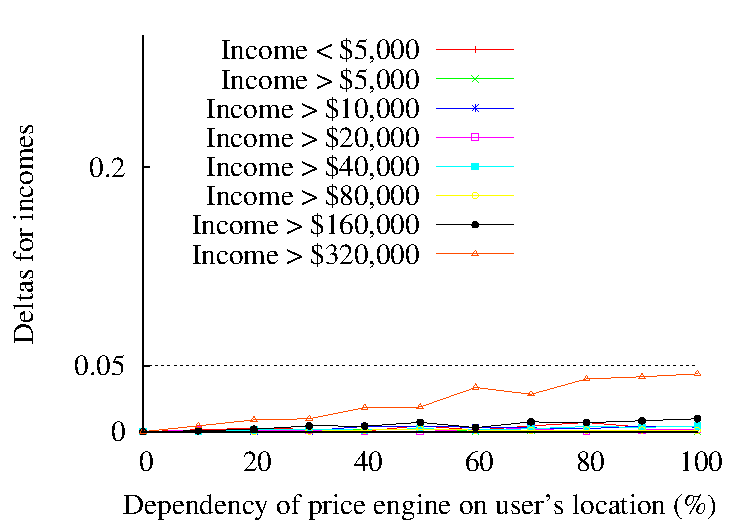
\includegraphics[width=0.45\textwidth]
  {\detokenize{results/income_discrimination_on_location_dependency}}
  \caption{\textbf{...} ...}
 \label{fig:}
\end{figure}

\begin{figure}[t]
 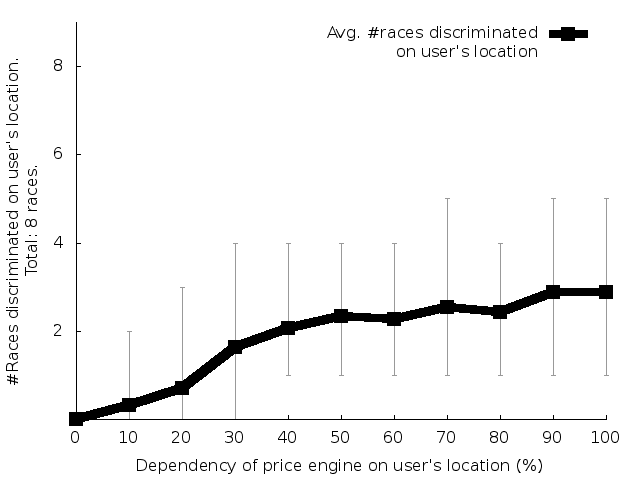
\includegraphics[width=0.45\textwidth]
  {\detokenize{results/race_discrimination_on_location_dependency}}
  \caption{\textbf{...} ...}
 \label{fig:}
\end{figure}

\begin{figure}[t]
 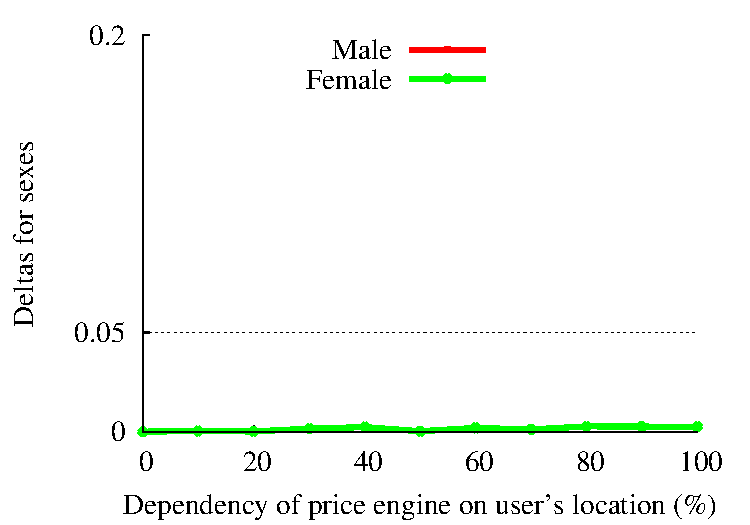
\includegraphics[width=0.45\textwidth]
  {\detokenize{results/sex_discrimination_on_location_dependency}}
  \caption{\textbf{...}...}
 \label{fig:}
\end{figure}

\begin{figure}[t]
 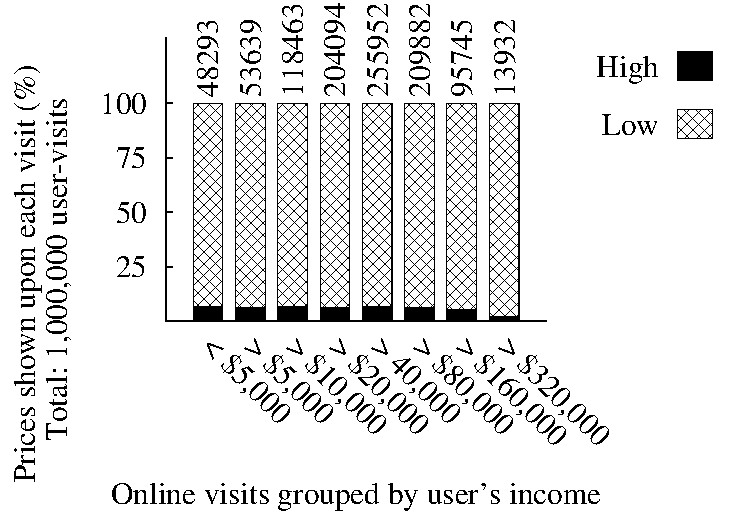
\includegraphics[width=0.45\textwidth]
  {\detokenize{results/income_discrimination_on_proportional}}
  \caption{\textbf{...} ...}
 \label{fig:}
\end{figure}

\begin{figure}[t]
 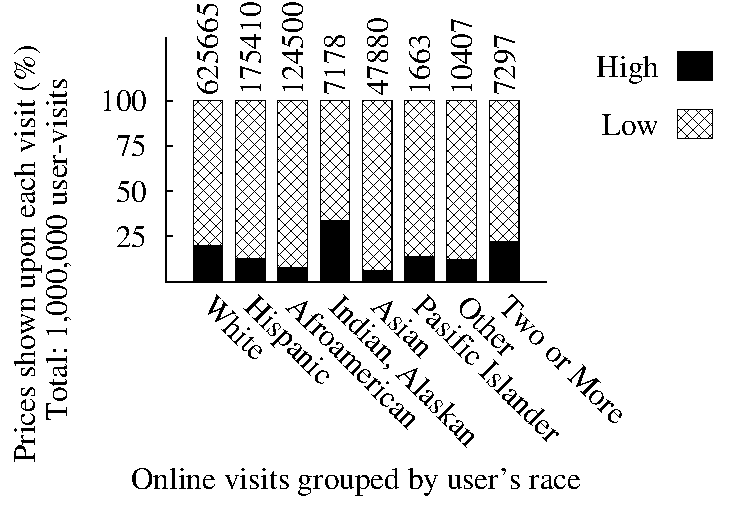
\includegraphics[width=0.45\textwidth]
  {\detokenize{results/race_discrimination_on_proportional}}
  \caption{\textbf{...} ...}
 \label{fig:}
\end{figure}

\begin{figure}[t]
 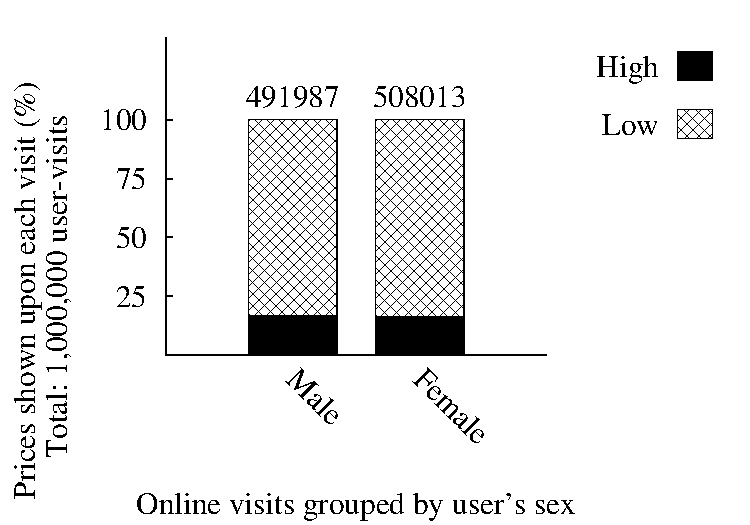
\includegraphics[width=0.45\textwidth]
 {\detokenize{results/sex_discrimination_on_proportional}}
  \caption{\textbf{...}...}
 \label{fig:}
\end{figure}

\begin{figure}[t]
 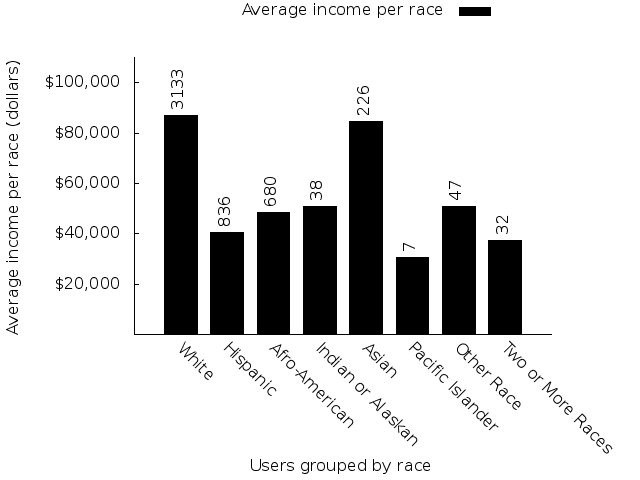
\includegraphics[width=0.45\textwidth]
 {\detokenize{results/income_per_race}}
  \caption{\textbf{...}...}
 \label{fig:}
\end{figure}
